
\section{Architecture and Implementation}

This chapter describes the architecture and the implementation of the traffic sign detection of an autonomous car in the neurorobotics platform. The implementation part will be described as follows: 
\begin{itemize}
	\item Traffic signs detection
	\item Car control
	\item Environment setup: street and car model
	\item Traffic signs 
\end{itemize}

\subsection{Detection of Traffic Signs}

To implement the detection of traffic signs a neural network model was trained. Training was performed on pre-trained model from the tensorflow object detection models zoo, namely ssdlite mobilenet v2 model pre-trained on COCO dataset\cite{DBLP:journals/corr/HuangRSZKFFWSG016}. MobileNets family of computer vision models is designed for resource constraint environments while maintaining high accuracy. They target mobile and embedded devices, their careful use of resources allows us to achieve satisfactory inference speed when running the detection in NRP, which does not support the use of graphics processing units at the moment. The model also implements SSDLite framework, which is a mobile friendly version of the regular SSD framework\cite{DBLP:journals/corr/abs-1801-04381}. This use of multibox detector method allows the model to perform localization of objects, which allows us to get the bounding boxes of the traffic signs. 


The dataset for training was fully generated without using existing traffic signs datasets. One image per each traffic sign used in the experiment was pasted on backgrounds, which were images randomly drawn from the COCO dataset. By providing sufficiently many and diverse images (not semantically related to the traffic scenes) we attempt to make our model generalize well in any environment. 3000 (three thousand) images per each traffic sign was generated as well as automatically produced annotation, which contained the class of the image and location of the traffic sign in the image by providing x coordinate minimum and maximum and y coordinate minimum and maximum. To make the detection more robust several random modifications were applied to signs in each image, such as perspective deformation, brightness change, blur and noise. In \ref{fig:img} we can see an example of one image from a total of 9000 images dataset.

\begin{figure}
  \centering
  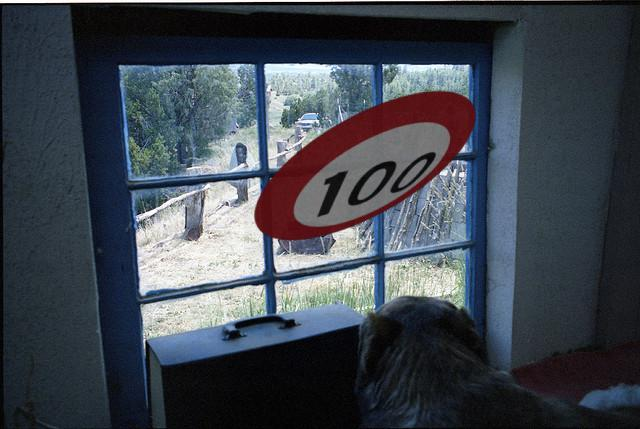
\includegraphics[width=0.7\textwidth]{chapter/images/img-1.jpg}
  \caption{Example of an image generated to train the neural network model}
  \label{fig:img}
\end{figure}


After training was performed several model checkpoints were tested in NRP and the best performing model was selected by simple observation of the performance. The current version of the model was achieved at step 18999 with the batch of 16 images, which is less than 37 epochs. The batch size was constrained by the GPU's memory on the personal computer used for training. Hyperparameters such as learning rate were used from the default training configuration from the tensorflow object detection api. Training script and config file, as well as dataset generation script will be submitted as a project deliverable. 8 percent of images were used as validation set, breaking down the 9000 images into 720 images validation and 8280 images training set.


Inference graph was saved in the .opt/graph\_def directory of the NRP container as well as accompanying label map. The training was performed using tensorflow and the transfer function of our experiment makes use of tensorflow api. Object detector transfer function runs a tensorflow session, which returns the number of detections in an image it gets from the car's camera, scores for these detections, classes and boxes, where boxes are maximum and minimum x and y coordinates of the detected traffic signs. Afterwards the square of the bounding box for each detection is calculated to determine, which of the signs has the biggest bounding box, assuming that this sign is the closest one to the car. After such sign is determined it is passed to the car's transfer function, where the car's logic is implemented. 

\subsection{Speed Limit Sign Section}

The traffic sign model in the experiment is the most important part of the environment as it directly influences the car’s decision making. For the simplicity, only speed limit signs are to be used because this sign can already lead to a visible effect (acceleration or deceleration) on the car. The traffic sign cognition function of the car can therefore be obviously proved. 



The technique used in the car to recognize the traffic sign is neural network. And the training dataset of the neural network is a fully generated dataset. As this dataset doesn’t include all types of speed limit signs, the model should include the right speed limit model (rather than a random one) so that the trained model in the car can detect and recognize the speed limit sign in the right way. In the experiment, speed limit signs for 100 km/h and 20 km/h are used.



A compatible model in NRP is defined mainly by three files: ``limit20.dae'', ``model.config'', and ``model.sdf''. The ``model.config'' file configures the author, model name, model version and description. The ``model.sdf defines'' the physical property of the model like geometry and collision property. The ``limit20.dae'' specifies the property of the speed limit sign in detail. For example, texture, material, and relative position of the traffic signs are defined in this file.



To speed up the model building, a reference model in ``.skp'' format is downloaded from the internet. To change it into a ``.dae'' format which is compatible with NRP, the 3D modeling software ``Sketchup'' in operating system Windows 10 (this software is not supported in Ubuntu) is used to convert the file to ``.dae'' format. The following operations are implemented in Ubuntu 16.04 operating system. 



After having the above files, the scripts are edited according to the model physical property, model name, model directory, and reference pictures. A new ``.sdf'' file is created to configure the geometry, link, collision property with the use of the ``.dae'' file. 

After implementing the above steps, the model should be available in the NRP platform.





\begin{table}[htpb]
	\caption[Example table]{An example for a simple table.}\label{tab:sampleA}
	\centering
	\begin{tabular}{l l l l}
		A & B & C & D \\
		\cline{1-4}	
		1 & 2 & 1 & 2 \\
		2 & 3 & 2 & 3 \\
	\end{tabular}
\end{table}



